\documentclass[nojss]{jss}\usepackage[]{graphicx}\usepackage[]{color}
%% maxwidth is the original width if it is less than linewidth
%% otherwise use linewidth (to make sure the graphics do not exceed the margin)
\makeatletter
\def\maxwidth{ %
  \ifdim\Gin@nat@width>\linewidth
    \linewidth
  \else
    \Gin@nat@width
  \fi
}
\makeatother

\definecolor{fgcolor}{rgb}{0.345, 0.345, 0.345}
\newcommand{\hlnum}[1]{\textcolor[rgb]{0.686,0.059,0.569}{#1}}%
\newcommand{\hlstr}[1]{\textcolor[rgb]{0.192,0.494,0.8}{#1}}%
\newcommand{\hlcom}[1]{\textcolor[rgb]{0.678,0.584,0.686}{\textit{#1}}}%
\newcommand{\hlopt}[1]{\textcolor[rgb]{0,0,0}{#1}}%
\newcommand{\hlstd}[1]{\textcolor[rgb]{0.345,0.345,0.345}{#1}}%
\newcommand{\hlkwa}[1]{\textcolor[rgb]{0.161,0.373,0.58}{\textbf{#1}}}%
\newcommand{\hlkwb}[1]{\textcolor[rgb]{0.69,0.353,0.396}{#1}}%
\newcommand{\hlkwc}[1]{\textcolor[rgb]{0.333,0.667,0.333}{#1}}%
\newcommand{\hlkwd}[1]{\textcolor[rgb]{0.737,0.353,0.396}{\textbf{#1}}}%

\usepackage{framed}
\makeatletter
\newenvironment{kframe}{%
 \def\at@end@of@kframe{}%
 \ifinner\ifhmode%
  \def\at@end@of@kframe{\end{minipage}}%
  \begin{minipage}{\columnwidth}%
 \fi\fi%
 \def\FrameCommand##1{\hskip\@totalleftmargin \hskip-\fboxsep
 \colorbox{shadecolor}{##1}\hskip-\fboxsep
     % There is no \\@totalrightmargin, so:
     \hskip-\linewidth \hskip-\@totalleftmargin \hskip\columnwidth}%
 \MakeFramed {\advance\hsize-\width
   \@totalleftmargin\z@ \linewidth\hsize
   \@setminipage}}%
 {\par\unskip\endMakeFramed%
 \at@end@of@kframe}
\makeatother

\definecolor{shadecolor}{rgb}{.97, .97, .97}
\definecolor{messagecolor}{rgb}{0, 0, 0}
\definecolor{warningcolor}{rgb}{1, 0, 1}
\definecolor{errorcolor}{rgb}{1, 0, 0}
\newenvironment{knitrout}{}{} % an empty environment to be redefined in TeX

\usepackage{alltt}

%\usepackage{setspace}
% \usepackage[sc]{mathpazo}
\usepackage{amsmath}
% %\usepackage{geometry} 
% %\geometry{verbose,tmargin=1.25cm,bmargin=1.25cm,lmargin=1.25cm,rmargin=1.25cm}
% \setcounter{secnumdepth}{2}
% \setcounter{tocdepth}{2}

\usepackage{longtable}
\usepackage{colortbl, xcolor}
\usepackage{booktabs}

%%%%%%%%%%%%%%%%%%%%%%%%%%%%%%
%% declarations for jss.cls %%
%%%%%%%%%%%%%%%%%%%%%%%%%%%%%%
%\VignetteEngine{knitr::knitr}
%\VignetteIndexEntry{ggRandomForests}
%\VignetteIndexEntry{Random Forests for Survival ggRandomForests packages}                                          
%\VignetteKeywords{random forest, survival, VIMP, minimal depth}                                                                   
%\VignetteDepends{ggRandomForests}                                      
%\VignettePackage{ggRandomForests} 

%% almost as usual
\author{John Ehrlinger 
\and Eugene H. Blackstone\\Cleveland Clinic}

\title{\pkg{ggRandomForests}: Random Forests for Survival}

%% for pretty printing and a nice hypersummary also set:
\Plainauthor{Ehrlinger et.\ al.} %% comma-separated
\Plaintitle{ggRandomForests: Random Forests for Survival} %% without formatting
\Shorttitle{Random Forests for Survival}

%% an abstract and keywords
\Abstract{ 
Random Forests~\citep{Breiman:2001} (RF) are a fully non-parametric statistical method requiring no distributional assumptions on covariate relation to the response. RF are a robust, nonlinear technique that optimizes predictive accuracy by fitting an ensemble of trees to stabilize model estimates. Random Forests for survival~\citep{Ishwaran:2007a,Ishwaran:2008} (RF-S) are an extension of Breiman's RF techniques to survival settings, allowing efficient non-parametric analysis of time to event data. The \pkg{randomForestSRC} package~\citep{Ishwaran:RFSRC:2014} is a unified treatment of Breiman's random forests for survival, regression and classification problems.

Predictive accuracy make RF an attractive alternative to parametric models, though complexity and interpretability of the forest hinder wider application of the method. We introduce the \pkg{ggRandomForests} package, tools for creating and plotting data structures to visually understand random forest models grown in \proglang{R} with the \pkg{randomForestSRC} package. The \pkg{ggRandomForests} package is structured to extract intermediate data objects from \pkg{randomForestSRC} objects and generate figures using the \pkg{ggplot2}~\citep{Wickham2009} graphics package.

This document is formatted as a tutorial for using the \pkg{randomForestSRC} for building random forests for survival and \pkg{ggRandomForests} package for investigating how the forest is constructed. This tutorial uses the Primary Biliary Cirrhosis (PBC) Data from the Mayo Clinic~\citep{fleming:1991} available in the  \pkg{randomForestSRC} package. We use Variable Importance measure (VIMP)~\citep{Breiman:2001} as well as  Minimal Depth~\citep{Ishwaran:2010}, a property derived from the construction of each tree within the forest, to assess the impact of variables on forest prediction. We will also demonstrate the use of variable dependence plots~\citep{Friedman00greedyfunction} to aid interpretation RF results in different response settings. We also will investigate interactions between covariates to demonstrate the strength of the Random Forest method in survival settings.
}
\Keywords{random forest, survival, VIMP, minimal depth, \proglang{R}, \pkg{randomForestSRC}}
\Plainkeywords{random forest, survival, VIMP, minimal depth, R, randomForestSRC}
%% at least one keyword must be supplied

%% publication information
%% NOTE: Typically, this can be left commented and will be filled out by the technical editor
%% \Volume{13}
%% \Issue{9}
%% \Month{September}
%% \Year{2004}
%% \Submitdate{2004-09-29}
%% \Acceptdate{2004-09-29}

%% The address of (at least) one author should be given
%% in the following format:
\Address{
John Ehrlinger\\
Quantitative Health Sciences\\
Lerner Research Institute\\
Cleveland Clinic\\
9500 Euclid Ave\\
Cleveland, Ohio 44195\\
%  Telephone: +41/0/44634-4643 \\
%  Fax: +41/0/44634-4386 \\
E-mail: \email{john.ehrlinger@gmail.com}\\
URL: \url{http://www.lerner.ccf.org/qhs/people/ehrlinj/}
}

%% It is also possible to add a telephone and fax number
%% before the e-mail in the following format:
%% Telephone: +43/1/31336-5053
%% Fax: +43/1/31336-734

%% for those who use Sweave please include the following line (with % symbols):
%% need no \usepackage{Sweave.sty}

%% end of declarations %%%%%%%%%%%%%%%%%%%%%%%%%%%%%%%%%%%%%%%%%%%%%%%



\IfFileExists{upquote.sty}{\usepackage{upquote}}{}
\begin{document}
% -----------------------------------------------------
\section{About this document}
% -----------------------------------------------------
This document is an introduction to the \pkg{ggRandomForests} \proglang{R} package. The aim of this introduction is to provide a detailed user guide to \pkg{ggRandomForests} as well as provide a tutorial to building a Random Forest Survival model with the \pkg{randomForestSRC} package. Our attempt is to build simple, reproducible worked examples with the Primary Biliary Cirrhosis (PBC) Data from the Mayo Clinic.

This document is available as a vignette within \pkg{ggRandomForests} package, available from the Comprehensive \proglang{R} Archive Network via \url{http://CRAN.R-project.org/package=ggRandomForests}.

% -----------------------------------------------------
\section{Introduction} \label{S:introduction}
% -----------------------------------------------------

Random Forests~\citep{Breiman:2001} (RF) are a robust, non-parametric statistical method that optimizes predictive accuracy by averaging an ensemble of tree models. Random Forests are not parsimonious, utilizing all provided variables in predicting the specified outcome. It does not require prior knowledge of the parametric relation of variables (linearity or non-linearity) to the response, or of interactions between variables. RF chooses the most important variables by assessing variable impact on the predictive ability of the forest of trees.

A Random Forest is built up by bagging~\citep{Breiman:1996} a collection of classification and regression trees~\citep{cart:1984} (CART). The method uses a set of $B$ bootstrap~\citep{bootstrap:1994} samples, growing a set of independent tree models on each sub-sample of the population. Trees are grown by recursively partitioning the population based on optimization of a split rule over the $p$ dimensional covariate space. At each split, a subset of  $m \le p$ candidate variables are chosen for the splitting. Each node is split into two daughter nodes by maximizing the separation of observations according the split rule. In regression trees, node impurity is measured by mean squared error, whereas in classification problems, the Gini index is used~\citep{FriedmanGreedyfunction:2000}. Each subsequent daughter node is then split until the process reaches the stopping criteria of either node purity or node member size defining the set of terminal (unsplit) nodes for the tree. Random Forests sort each observation into one unique terminal node per tree. The Random Forest estimate for each observation is calculated by aggregation, averaging (regression) or votes (classification), the terminal node results across the collection of $B$ trees. 

One advantage of Random Forests is a built in generalization error estimate. Each bootstrap sample selects approximately $63.2\%$ of the population  on average. The remaining $36.8\%$ of observations, the Out-of-Bag~\citep{BreimanOOB:1996e} (OOB) sample, can be used as a hold out test set for each tree. An OOB prediction error estimate can be calculated for each observation by predicting the response over the set of trees which were NOT trained with that particular observation. Out-of-Bag prediction error estimates have been shown to be nearly identical to $n$--fold cross validation estimates~\citep{StatisticalLearning:2009}. This feature of Random Forests allows us to obtain both model fit and validation in one pass of the algorithm.

\subsection{Random Forests for Survival}\label{S:rfs}
Random Forests for survival~\citep{Ishwaran:2007,Ishwaran:2008} (RF-S) are an extension of~\cite{Breiman:2001} Random Forests for right censored time to event data. A forest of survival trees is grown using a log-rank splitting rule to select the optimal candidate variables. Survival estimate for each observation are constructed with a Kaplan--Meier (KM) estimator within each terminal node, at each event time. 

Random Forests for survival adaptively discover nonlinear effects and interactions and are fully nonparametric. Averaging over trees, with randomizing while growing a tree, enables RF-S to approximate complex survival functions, including non-proportional hazards, while maintaining low prediction error. \cite{Ishwaran:2010a} showed that RF-S is uniformly consistent and that survival forests have a uniform approximating property in finite-sample settings, a property not possessed by individual survival trees.

\subsection{ggRandomForests}
The \pkg{randomForestSRC} package is a mature analysis and research random forest implementation under rapid development. The package includes diagnostic  and post processing functions for analysis and visualizations of randomForest model properties. However, in our research we frequently found it difficult to manipulate the standard figures directly produced with the \pkg{randomForestSRC} package. 

In order to simplify these manipulations, we developed the \pkg{ggRandomForests} package. We attempted to follow two design principles in this development:
\begin{itemize}
\item Model/View separation: The package originally designed to generating \pkg{ggplot2}~\cite{Wickham2009} figures for random forest objects. However, some users would prefer to use other graphing methods within \proglang{R} or outside of it. To help users, we separate the data generation and the figure generation into two separate operations. 

\item Modular: We strive to create a modular design by following the \emph{do one thing well} philosphy. Each function operates on one \pkg{randomForestSRC} object to create only one data object or figure type.
\end{itemize}

To demonstrate using the \pkg{ggRandomForests} package, we organize this document as follows. In Section~\ref{S:rfsrcGrow} we outline growing a random forest for each of the classification, regression and survival settings with the \pkg{randomForestSRC} package. We use the \pkg{ggRandomForests} package to begin exploring random forest convergence and prediction. In Section~\ref{S:variableIdentification} we discuss how variables contribute to the random forest prediction using the Variable Importance (VIMP) and Minimal Depth measures.

Once we have an idea which variables are most informative in minimizing forest prediction error, we turn our focus to how the variables are related to the forest prediction. Because Random Forests are non-linear and non-parametric predictors, we can use variable dependence (Section~\ref{S:variableDependence}) to examine where each observation contributes to model prediction as a function of specific covariate values. Partial dependence (Section~\ref{S:partialDependence}) gives us a risk adjust view of the predictor dependence on a variable. We then find two way interactions using minimal depth in Section~\ref{S:interactions} and use conditional plots in Section~\ref{S:coplots} to look variable interactions in an intuitive manner.

\section{Data Summary: Primary Biliary Cirrhosis (PBC) Data}

Data from the Mayo Clinic trial in primary biliary cirrhosis (PBC) of the liver conducted between 1974 and 1984. A total of 424 PBC patients, referred to Mayo Clinic during that ten-year interval, met eligibility criteria for the randomized placebo controlled trial of the drug D-penicillamine. The first 312 cases in the data set participated in the randomized trial and contain largely complete data.



% latex table generated in R 3.1.2 by xtable 1.7-4 package
% Mon Dec  1 16:51:25 2014
\begin{table}[ht]
\centering
{\footnotesize
\begin{tabular}{rll}
  \toprule
 & label & type \\ 
  \midrule
days & survival time in days & integer \\ 
   \rowcolor[gray]{0.95}status & censoring indicator & logical \\ 
  treatment & 1=D-penicillamine, 2=placebo & factor \\ 
   \rowcolor[gray]{0.95}age & age in days & numeric \\ 
  sex & 0=female, 1=male & logical \\ 
   \rowcolor[gray]{0.95}ascites & presence of asictes & logical \\ 
  hepatom & presence of hepatomegaly & logical \\ 
   \rowcolor[gray]{0.95}spiders & presence of spiders & logical \\ 
  edema & presence of edema & factor \\ 
   \rowcolor[gray]{0.95}bili & serum bilirubin in mg/dl & numeric \\ 
  chol & serum cholesterol in mg/dl & integer \\ 
   \rowcolor[gray]{0.95}albumin & albumin in gm/dl & numeric \\ 
  copper & urine copper in ug/day & integer \\ 
   \rowcolor[gray]{0.95}alk & alkaline phosphatase in U/liter & numeric \\ 
  sgot & SGOT in U/ml & numeric \\ 
   \rowcolor[gray]{0.95}trig & triglicerides in mg/dl & integer \\ 
  platelet & platelets per cubic ml/1000 & integer \\ 
   \rowcolor[gray]{0.95}prothrombin & prothrombin time in seconds & numeric \\ 
  stage & histologic stage of disease & factor \\ 
   \rowcolor[gray]{0.95} \bottomrule
\end{tabular}
}
\caption{PBC Data field descriptions} 
\label{T:dataLabs}
\end{table}


%' Figure~\ref{fig:dtaViewCat} and~\ref{fig:dtaView} are included to verify the data import step. 
%' 
%' <<dtaViewCat, fig.cap="Categorical Variable measures over time.", fig.width=7.5, fig.height=4>>=
%' dta.tmp<-pbc[,c(which(cls == "factor"),
%'                 which(cls=="logical"), 
%'                    which(colnames(pbc) %in% c("age")))]
%' plt.dta <- dta.tmp %>% gather(variable, value, -age)
%' 
%' dtaView<- ggplot(plt.dta,aes(x=age, fill=value)) + 
%'   geom_histogram(binwidth=5, color="black")+
%'   labs(x="Age", y="")+
%'   facet_wrap(~variable, ncol=3)+
%'   theme(legend.position="none") +
%'   scale_fill_brewer(palette = "Paired", na.value="lightgrey")
%' 
%' suppressWarnings(show(dtaView))
%' 
%' @
%' 
%' <<dtaView, fig.cap="Continuous Variable measures over time.", fig.width=7.5, fig.height=4>>=
%' dta.tmp <- pbc[,c(which(cls == "numeric"),which(cls == "integer"), 
%'                      which(colnames(pbc)=="status"))]
%' 
%' plt.dta <- dta.tmp %>% gather(variable, value, -age, -status)
%' 
%' dtaView<- ggplot(plt.dta,aes(x=age, y=value, color=status, shape=status)) + 
%'   geom_point(alpha=alpha)+
%'   geom_rug(aes(x=age), data=plt.dta %>% filter(is.na(value)))+
%'   labs(x="Age", y="")+
%'   facet_wrap(~variable,scales = "free_y", ncol=3)+
%'   scale_color_manual(values=strCol, na.value = "black", drop=FALSE,
%'                      labels=event.labels)+
%'   scale_shape_manual(values=event.marks, labels=event.labels)+
%'   theme(legend.position="none")
%' 
%' suppressWarnings(show(dtaView))
%' @

% \doublespacing
\section{Growing the Random Forest}
\begin{knitrout}\footnotesize
\definecolor{shadecolor}{rgb}{0.969, 0.969, 0.969}\color{fgcolor}\begin{kframe}
\begin{verbatim}
R> pbc_rf <- rfsrc(Surv(days, status) ~ ., data = pbc, 
+                   ntree = 2000,
+                   na.action="na.impute", 
+                   fast.restore = TRUE)
\end{verbatim}
\end{kframe}
\end{knitrout}

\begin{knitrout}\footnotesize
\definecolor{shadecolor}{rgb}{0.969, 0.969, 0.969}\color{fgcolor}\begin{kframe}
\begin{verbatim}
                         Sample size: 276
                    Number of deaths: 111
                     Number of trees: 500
          Minimum terminal node size: 3
       Average no. of terminal nodes: 54.212
No. of variables tried at each split: 5
              Total no. of variables: 17
                            Analysis: RSF
                              Family: surv
                      Splitting rule: logrank *random*
       Number of random split points: 10
                          Error rate: 16.67%
\end{verbatim}
\end{kframe}
\end{knitrout}

Figure~\ref{fig:rfsrc-plot} shows the predicted survival from an RF-S model, where censored device prediction is colored in blue, and devices experiencing a thrombosis event are colored in red.  
\begin{knitrout}\footnotesize
\definecolor{shadecolor}{rgb}{0.969, 0.969, 0.969}\color{fgcolor}\begin{figure}[!htpb]

{\centering 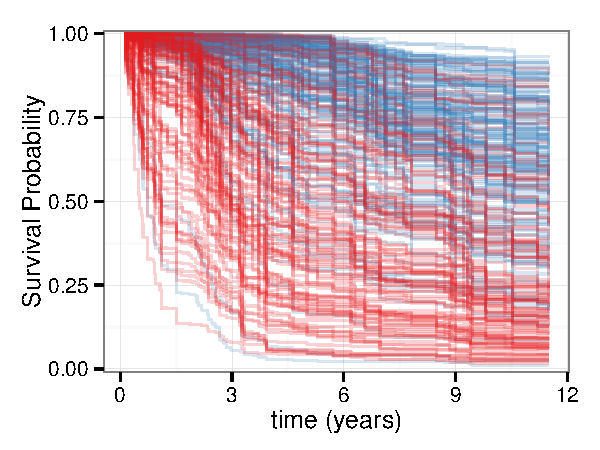
\includegraphics[width=\maxwidth]{figure/rfs-rfsrc-plot-1} 

}

\caption[PBC Survival]{PBC Survival\label{fig:rfsrc-plot}}
\end{figure}


\end{knitrout}

\section{Variable Selection}
Unlike in the linear model settings, Random Forests does not require explicitly specify the functional form of the covariates to the response. Instead, we ascertain which variables contribute to the Random Forest estimates by querying the forest for variable usage. 

\subsection{Variable Importance}\label{S:vimp}
Unlike in the linear model settings, Random Forests does not require explicitly specify the functional form of the covariates to the response. Instead, we ascertain which variables contribute to the Random Forest estimates by querying the forest for variable usage. 

Variable importance (VIMP) was originally defined in CART using a measure involving surrogate variables (see Chapter 5 of~\cite{cart:1984}). The most popular VIMP method to date, adopts a prediction error approach involving "noising-up" a variable. VIMP for a variable $x_v$ is the difference between prediction error when $x_v$ is noised up by permuting its value randomly, compared to prediction error under the original predictor~\citep{Breiman:2001,liaw:2002,Ishwaran:2007,Ishwaran:2008}.

Since VIMP is the absolute difference between prediction errors before and after permutation, a large VIMP value indicates that misspecification of that variable detracts from the predictive accuracy of the forest. VIMP close to zero indicates the variable contributes nothing to predictive accuracy, and negative values indicate the predictive accuracy improves when the variable is mispecified. In the later case, we assume noise is more informative than the variable. As such, we ignore variables with negative and near zero values of VIMP, relying on large positive values to indicate that the predictive power of the forest is dependent on those variables. 

In Figure~\ref{fig:rf-vimp}, we plot VIMP measures for each of the variables used to grow the forest estimates of Figure~\ref{fig:rfsrc-plot}. Variables are shown in VIMP rank order, largest (op\_yr) at the top, to smallest (iv\_lospr) at the bottom. In this case, we would focus attention on the top three variables (op\_yr (surgical date), ld and devno).
\begin{knitrout}\footnotesize
\definecolor{shadecolor}{rgb}{0.969, 0.969, 0.969}\color{fgcolor}\begin{kframe}
\begin{verbatim}
R> plot.gg_vimp(pbc_rf)+
+   theme(legend.position="none")
\end{verbatim}
\end{kframe}\begin{figure}[!htpb]

{\centering 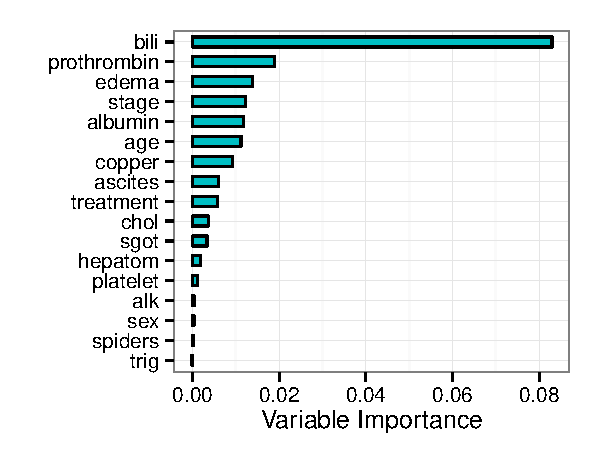
\includegraphics[width=\maxwidth]{figure/rfs-rf-vimp-1} 

}

\caption[Variable Importance]{Variable Importance\label{fig:rf-vimp}}
\end{figure}


\end{knitrout}

\subsection{Minimal Depth}\label{S:minimalDepth}
In VIMP, prognostic risk factors are determined by inspection of the forest, ranking the most important variables according to impact on predictive ability of the forest. An alternative method recognizes that most important variables for prediction are those that most frequently split nodes nearest to the trunks of the trees (ie, at the root node) since they partition the largest portions of the population. 

Node levels are numbered based on their relative distance to the trunk of the tree (ie. 0, 1, 2).  A measure of important risk factors is determined by averaging the depth of first split for each variable over all trees within the forest. Lower values of this measure indicate variables that split larger groups of patients. 

The maximal subtree for a variable $x$ is the largest subtree whose root node splits on $x$. Thus, all parent nodes of $x$'s maximal subtree have nodes that split on variables other than $x$. The largest maximal subtree possible is the root node. In general, however, there can be more than one maximal subtree for a variable. A maximal subtree may also not exist if there are no splits on the variable. The minimal depth of a maximal subtree (the first order depth) measures predictiveness of a variable $x$. It equals the shortest distance (the depth) from the root node to the parent node of the maximal subtree (zero is the smallest value possible). The smaller the minimal depth, the more impact $x$ has on prediction. The mean of the minimal depth distribution is used as the threshold value for deciding whether a variable's minimal depth value is small enough for the variable to be classified as strong. 

The minimal depth plot of Figure~\ref{fig:mindepth} is similar to the VIMP plot in Figure~\ref{fig:rf-vimp}, ranking variables from most important at the top (minimal depth measure), to least at the bottom (maximal minimal depth). Since the VIMP and Minimal Depth measures use different criteria, we expect the variable ranking to be slightly different. In this case, minimal depth indicates seven most important variables (op\_yr (surgical date), age, ld, ht, wt, iv\_lospr (length of stay) and inr). The vertical dashed line indicates the minimal depth threshold where smaller minimal depth values indicate higher importance and larger indicate lower importance.


\begin{knitrout}\footnotesize
\definecolor{shadecolor}{rgb}{0.969, 0.969, 0.969}\color{fgcolor}\begin{kframe}
\begin{verbatim}
R> pbc_vs <- var.select(pbc_rf)
R> ggMindepth <- gg_minimal_depth(pbc_vs)
R> 
R> ggMindepth
\end{verbatim}
\end{kframe}
\end{knitrout}

\begin{knitrout}\footnotesize
\definecolor{shadecolor}{rgb}{0.969, 0.969, 0.969}\color{fgcolor}\begin{kframe}
\begin{verbatim}
-----------------------------------------------------------
gg_minimal_depth
model size         : 12 
depth threshold    : 5.4163 

PE :[1] 16.671
-----------------------------------------------------------

Top variables:
            depth  vimp
bili        1.872 0.067
copper      2.450 0.023
albumin     2.714 0.008
chol        2.948 0.008
prothrombin 3.132 0.013
age         3.444 0.010
sgot        3.820 0.005
platelet    3.922 0.000
trig        3.960 0.001
alk         3.976 0.001
edema       4.402 0.016
stage       5.282 0.007
-----------------------------------------------------------
\end{verbatim}
\end{kframe}
\end{knitrout}

\begin{knitrout}\footnotesize
\definecolor{shadecolor}{rgb}{0.969, 0.969, 0.969}\color{fgcolor}\begin{figure}[!htpb]

{\centering 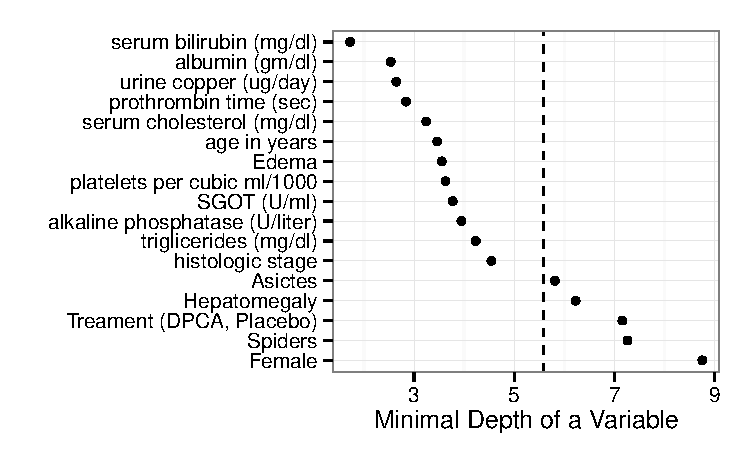
\includegraphics[width=\maxwidth]{figure/rfs-mindepth-plot-1} 

}

\caption[Minimal Depth Plot]{Minimal Depth Plot\label{fig:mindepth-plot}}
\end{figure}


\end{knitrout}


\section{Variable Dependence}\label{S:dependence}
Once we have an idea of which variables contribute to the predictive accuracy of the forest, it is useful to get some idea of form of this contribution. We use graphical methods to show the predicted response given dependence on covariates. We can plot the marginal effect of an covariate on the class probability (classification), response (regression), mortality (survival), or the expected years lost (competing risk) for a RF analysis. We plot the ensemble predicted value on the vertical axis and covariates along the horizontal axis.

\subsection{Marginal Dependence}\label{S:variableDependence}
\emph{Marginal variable dependence} plots the predicted response as a function of the covariate, showing each subject as a point on the plot. For classification and regression, this is straight forward predicting the response. In survival settings, we must account for the additional dimension of time. In this case, we plot the response at a specific time point of interest, for example survival at three months shown by the vertical dashed line in Figure~\ref{fig:rfsrc-plot3Mnth}. We take the predicted value of each curve at that time, and plot that against the covariate value for that observations, shown in Figure~\ref{fig:variable-plot}. Again censored cases are shown in blue circles, events are indicated by the red "x" symbols. Each predicted point is dependent on the full combination of all other covariates, not only on the covariate displayed in the dependence plot, so interpretation of these variable dependence plots can only be in general terms. The smooth loess line~\citep{cleveland:1981, cleveland:1988} indicates the trend of the prediction over surgical date progression.

\begin{knitrout}\footnotesize
\definecolor{shadecolor}{rgb}{0.969, 0.969, 0.969}\color{fgcolor}\begin{kframe}
\begin{verbatim}
R> ggRFsrc +
+   geom_vline(aes(xintercept=364.25), linetype="dashed")+
+   coord_cartesian(x=c(0,3*364.25))
\end{verbatim}
\end{kframe}\begin{figure}[!htpb]

{\centering 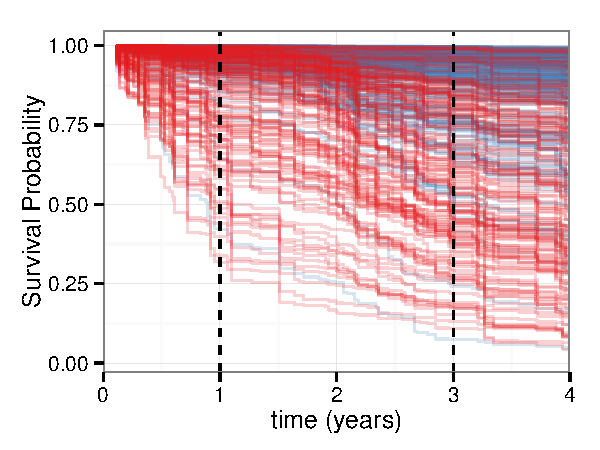
\includegraphics[width=\maxwidth]{figure/rfs-rfsrc-plot3Mnth-1} 

}

\caption[PBC Survival]{PBC Survival\label{fig:rfsrc-plot3Mnth}}
\end{figure}


\end{knitrout}

\begin{knitrout}\footnotesize
\definecolor{shadecolor}{rgb}{0.969, 0.969, 0.969}\color{fgcolor}\begin{kframe}
\begin{verbatim}
R> xvar <- pbc_vs$topvars[1:6]
R> ind=1
R> ggrf <- gg_variable(pbc_rf, time=c(1,3)*364.25, time.labels = c("1 Year", "3 Years"))
R> 
R> plot(ggrf, x_var = xvar[ind]) +
+   labs(y="Survival", x=dta.labs[which(rownames(dta.labs)==xvar[ind]), "label"])+
+   theme(legend.position="none")+
+   scale_color_manual(values=strCol, na.value = "black", drop=FALSE,
+                      labels=event.labels)+
+   scale_shape_manual(values=event.marks, labels=event.labels)
\end{verbatim}
\end{kframe}\begin{figure}[!htpb]

{\centering 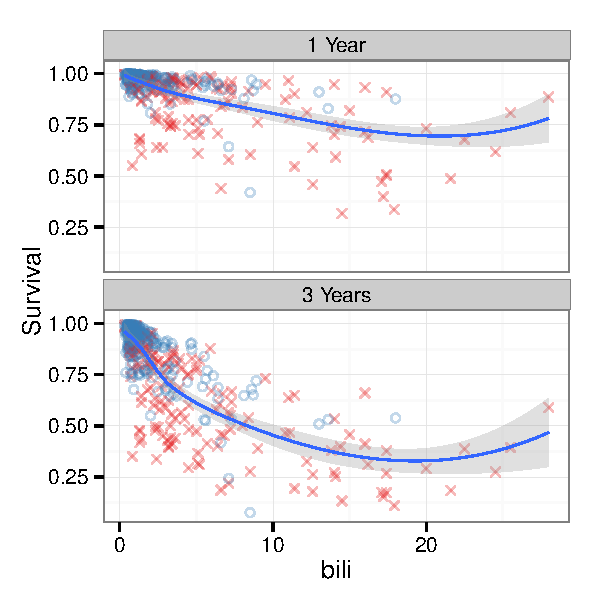
\includegraphics[width=\maxwidth]{figure/rfs-variable-plotbili-1} 

}

\caption[Variable dependence Survival vs]{Variable dependence Survival vs. Bilirubin\label{fig:variable-plotbili}}
\end{figure}


\end{knitrout}

\begin{knitrout}\footnotesize
\definecolor{shadecolor}{rgb}{0.969, 0.969, 0.969}\color{fgcolor}\begin{kframe}
\begin{verbatim}
R> plot(ggrf, x_var = xvar[2:6], panel=TRUE) +
+   labs(y="Survival")+
+   theme(legend.position="none")+
+   scale_color_manual(values=strCol, na.value = "black", drop=FALSE,
+                      labels=event.labels)+
+   scale_shape_manual(values=event.marks, labels=event.labels)
\end{verbatim}
\end{kframe}\begin{figure}[!htpb]

{\centering 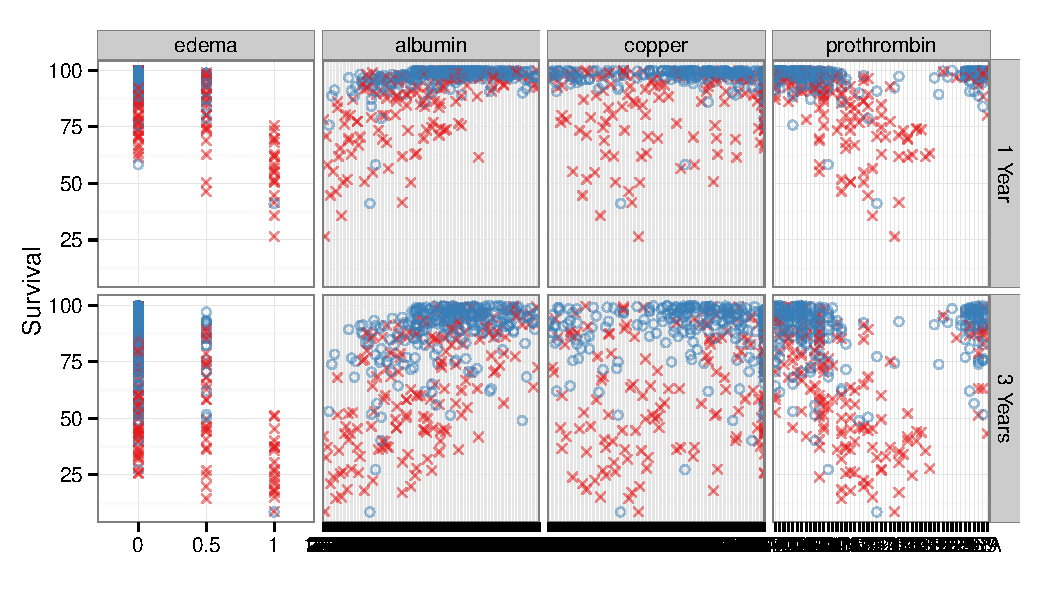
\includegraphics[width=\maxwidth]{figure/rfs-variable-plotCombines-1} 

}

\caption[Variable dependence Survival panel]{Variable dependence Survival panel\label{fig:variable-plotCombines}}
\end{figure}


\end{knitrout}

\subsection{Partial Dependence}\label{S:partialDependence}

\emph{Partial dependence plots} are a risk adjusted alternative to marginal variable dependence. Partial plots are generated by integrating out the effects of variables beside the covariate of interest. The figures are constructed by selecting points evenly spaced along the distribution of the X variable. For each of these values (X=x), we calculate the average Random Forest prediction over all other covariates in X by \eqref{E:partial}.
\begin{equation}
\tilde{f}(x) = \frac{1}{n} \sum_{i=1}^n \hat{f}(x, x_{i,o}),
\label{E:partial}
\end{equation}
where $\hat{f}$ is the predicted response from the random forest and $x_{i,o}$ is the value for all other covariates other than $X=x$ for the observation $i$~\citep{FriedmanGreedyfunction:2000}. Partial dependence plots in time to event settings are shown at specific time points, similar to variable dependence.

Figure~\ref{fig:pbc-partial-bili} shows the partial dependence of three month freedom from thrombosis on the surgical date covariate. 

\begin{knitrout}\footnotesize
\definecolor{shadecolor}{rgb}{0.969, 0.969, 0.969}\color{fgcolor}\begin{kframe}
\begin{verbatim}
R> pbc_prtl <- plot.variable(pbc_rf, surv.type="surv", time=364.25, 
+                       xvar.names=xvar, partial=TRUE,
+                       show.plots = FALSE)
R> pbc_prtl.3 <- plot.variable(pbc_rf, surv.type="surv", time=3*364.25, 
+                       xvar.names=xvar, partial=TRUE,
+                       show.plots = FALSE)
R> 
R> ggPrtl <- gg_partial(pbc_prtl)
R> ggPrtl.3 <- gg_partial(pbc_prtl.3)
R> 
R> ## Need a merge.gg_partial function to combine multiple time curves along variables.
R> ## pbc.prtl <- merge(ggPrtl, ggPrtl.3)
\end{verbatim}
\end{kframe}
\end{knitrout}




\begin{knitrout}\footnotesize
\definecolor{shadecolor}{rgb}{0.969, 0.969, 0.969}\color{fgcolor}\begin{kframe}
\begin{verbatim}
R> ind  <- 1
R> plot(ggPrtl[[ind]], se=FALSE)+
+   theme(legend.position=c(.2,.2))+
+   labs(y="Survival at 1 year", x=dta.labs[which(rownames(dta.labs)==xvar[ind]), "label"])+
+   scale_color_manual(values=strCol, na.value = "black", drop=FALSE,
+                      labels=event.labels)+
+   scale_shape_manual(values=event.marks, labels=event.labels)
\end{verbatim}
\end{kframe}\begin{figure}[!htpb]

{\centering 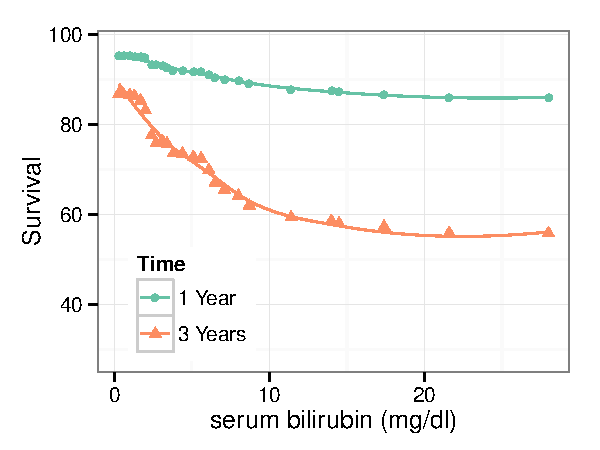
\includegraphics[width=\maxwidth]{figure/rfs-pbc-partial-bili-1} 

}

\caption[Risk adjusted Survival]{Risk adjusted Survival\label{fig:pbc-partial-bili}}
\end{figure}


\end{knitrout}

\section{Variable Interactions}\label{S:interactions}
Using the different variable dependence measures, we can calculate pairwise interactions for any pair of variables. 

Using minimal depth, we calculate the maximal subtree using the normalized minimal depth of variable $i$ relative to the root node (normalized with respect to the size of the tree) the maximal subtree interaction measure  is the normalized minimal depth of a variable $j$ wet the maximal subtree for variable $i$ (normalized wet the size of $i$'s maximal subtree). Smaller diagonal entries indicate predictive variables. Small interaction entries having small diagonal entries are a sign of an interaction between variable $i$ and $j$~\citep{Ishwaran_HighDimension:2010,Ishwaran_HighDimension:2011} 

By plotting the resulting interaction measures for each variable (Figure~\ref{fig:interaction}), we can detect the "most interactive" pairs, and develop conditional plots~\cite{chambers:1992,cleveland:1993}. These plots are similar to stratified results, arranged in a set of panels by the interactive variable of interest. 
\begin{knitrout}\footnotesize
\definecolor{shadecolor}{rgb}{0.969, 0.969, 0.969}\color{fgcolor}\begin{kframe}
\begin{verbatim}
R> pbc_interaction <- find.interaction(pbc_rf)
R> plot(gg_interaction(pbc_interaction), x_var=xvar[1])+
+   labs(y="Interactive Minimal Depth")
\end{verbatim}
\end{kframe}
\end{knitrout}
\begin{knitrout}\footnotesize
\definecolor{shadecolor}{rgb}{0.969, 0.969, 0.969}\color{fgcolor}\begin{figure}[!htpb]

{\centering 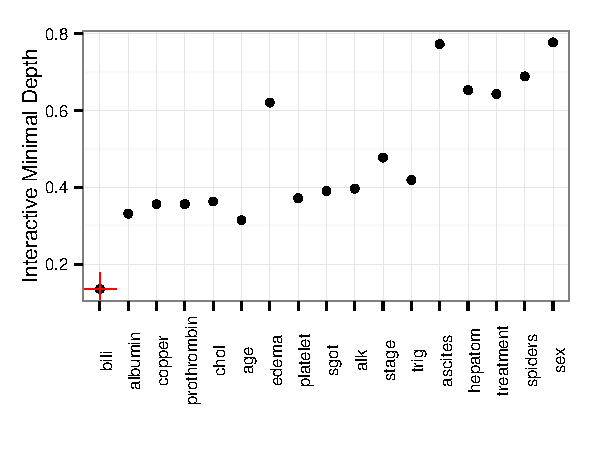
\includegraphics[width=\maxwidth]{figure/rfs-interaction-1} 

}

\caption[Minimal Depth interaction for Surgical Date]{Minimal Depth interaction for Surgical Date\label{fig:interaction}}
\end{figure}


\end{knitrout}

\subsection{Conditional Dependence Plots}



\section{Conclusion}


%\singlespacing
\bibliography{ggRandomForests}

\end{document}
